\section{Logical and Physical Database Design}
\label{appendix:database-design}

The Entity-Relationship Diagram in Section~\ref{sec:database-design} states what the main database holds and how its entities relate. The two views below restate that same structure at the levels beneath it: the logical design as the relations, attributes and keys the schema declares, and the physical design as what is actually created in PostgreSQL --- column types, indexes, and the constraints that enforce the model rather than merely describing it.

\subsection{Logical Database Design}

\begin{figure}[H]
    \centering
    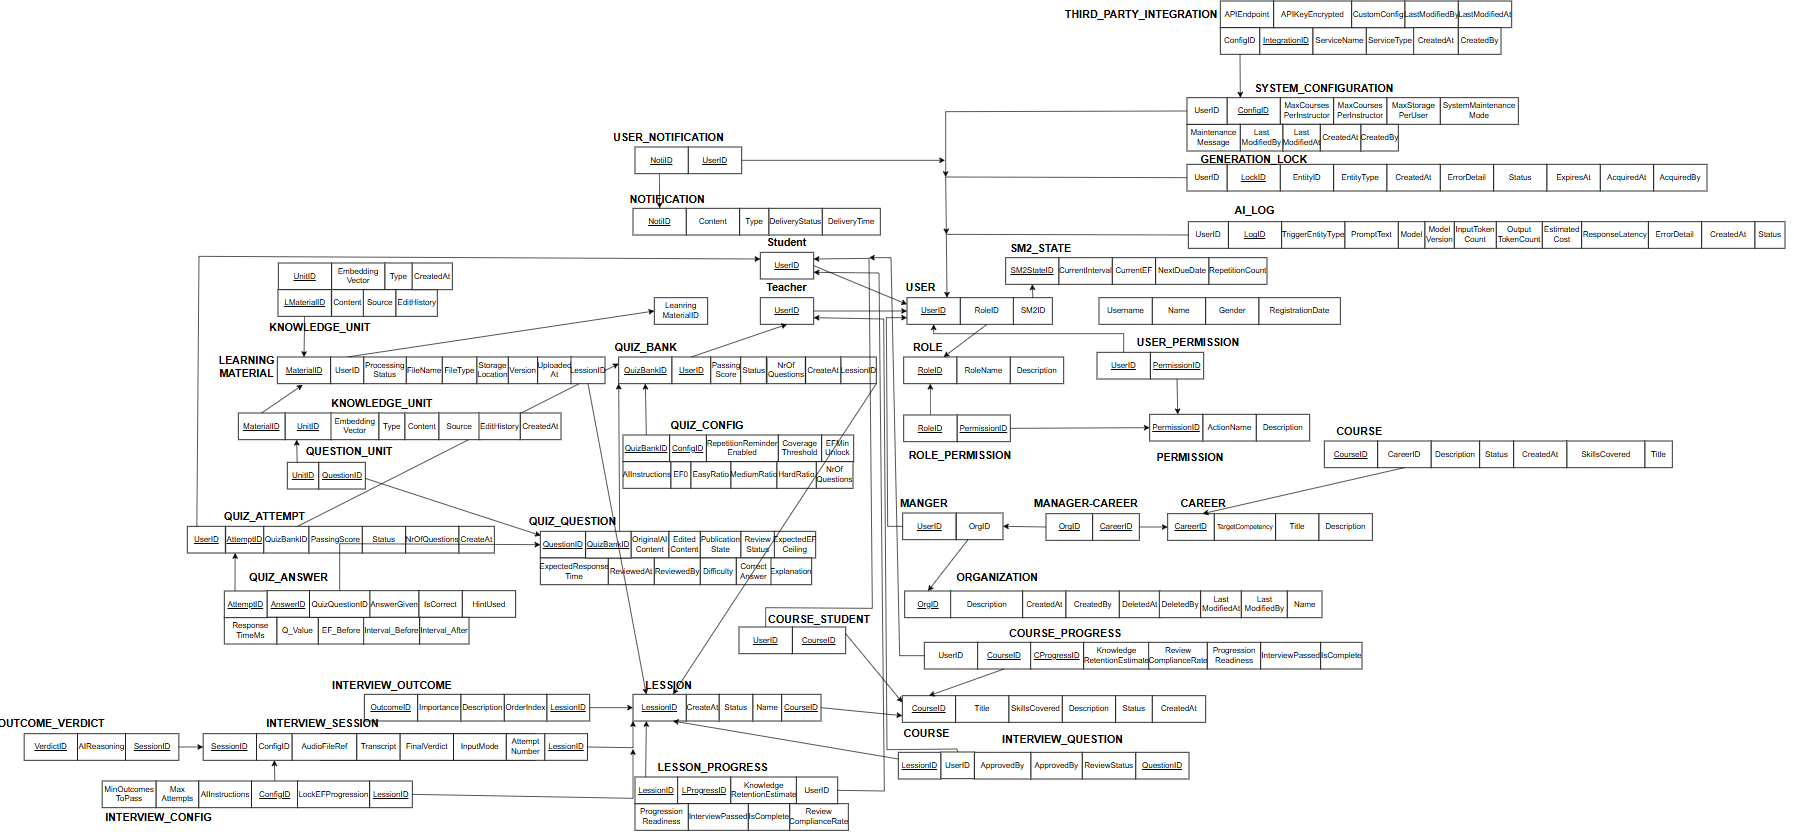
\includegraphics[width=\textwidth]{graphics/db-diagrams/LOGICAL_DESIGN.png}
    \caption{Logical Database Design}
    \label{fig:logical-db-design}
\end{figure}

\subsection{Physical Database Design}

\begin{figure}[H]
    \centering
    \includegraphics[width=\textwidth]{graphics/db-diagrams/PHYSICAL_DESIGN.pdf}
    \caption{Physical Database Design}
    \label{fig:physical-db-design}
\end{figure}
